% =========================================================================== %

\begin{frame}[t,plain]
\titlepage
\end{frame}

% =========================================================================== %\\

\begin{frame}{Christmas Settings}
%
\begin{columns}[T]
\column{.5\linewidth}
\vspace{-12pt}
\begin{center}
	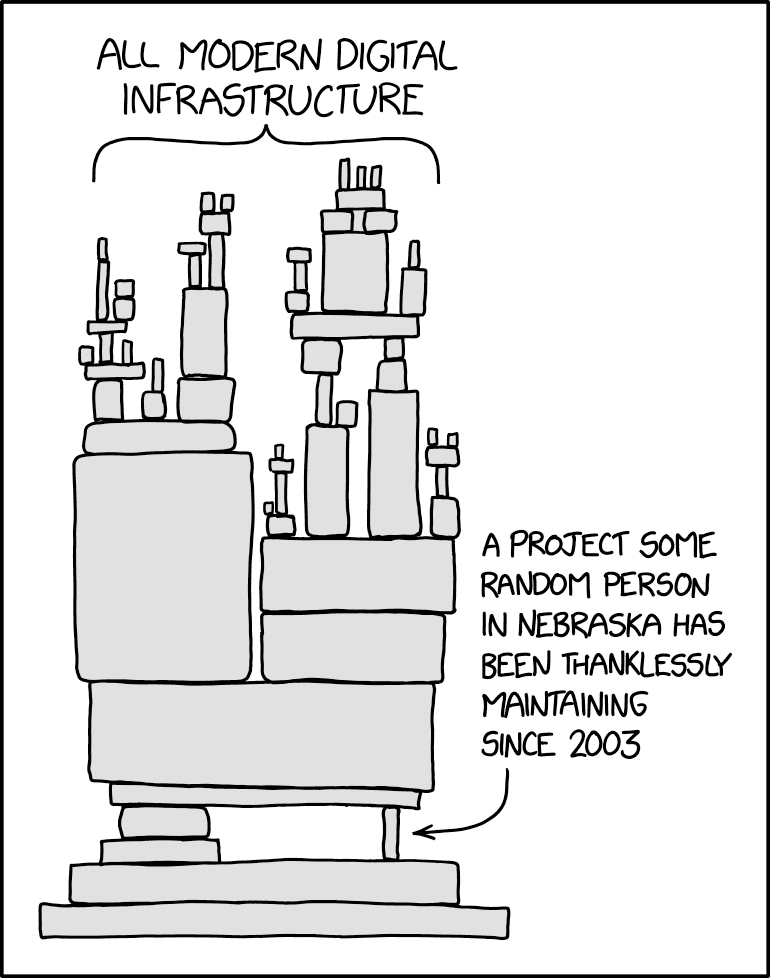
\includegraphics[width=.7\linewidth]{./gfx/11-xkcd-dependency}
\end{center}
%
\column{.5\linewidth}
\vspace{+40pt}
\begin{center}
	\emph{Someday ImageMagick will finally break for good and we'll have a long period of scrambling as we try to reassemble civilization from the rubble.}
	
	\vspace{12pt}
	Source: \url{https://xkcd.com/2347/}
\end{center}
\end{columns}
%
\end{frame}

% =========================================================================== %

\begin{frame}{Scope For Today}
%
\begin{itemize}
\item Compiling and Linking Libraries
	\begin{itemize}
	\item Multi-Module C/C++ Codes
	\item Static and Shared Libraries
	\item Invocation of the gcc/g++
	\end{itemize}
\item Loading C Libraries in Python
	\begin{itemize}
	\item Marshalling (Managing data representation)
	\item Package-like Modue Loader
	\item Name mangling or why C++ is different
	\end{itemize}
\item Automatization
	\begin{itemize}
	\item \todo{foo bar}
	\end{itemize}
\end{itemize}
%
\end{frame}

% =========================================================================== %

\begin{frame}{Compiling, Assembling and Linking}
%
\begin{itemize}
\item Every-day language\footnote{for nerds like us}: to compile = to translate source code into executable machine language
\item Uh, technically ...
	\begin{itemize}
	\item Compiling: translating a high-level language into a low-level language
	\item Assembling: creating \emph{object code} (essentially machine language fragments) from low-level language code
	\item Linking: combining object code files and libraries into a single executable file
	\end{itemize}
\item Object code files (\texttt{*.o})
	\begin{itemize}
	\item Binary / not human readable
	\item Essentially differs from executables by lacking a header
	\item Allows code-organization into modules and re-use without re-compiling and re-assembling
	\end{itemize}
\item Static Library
	\begin{itemize}
	\item Like a zip-file containing object files
	\end{itemize}
\end{itemize}
%
\end{frame}

% =========================================================================== %

\begin{frame}{Static Linkage to an Executable}
%
\begin{itemize}
\item Main actions
	\begin{itemize}
	\item Copy/Paste all object code into a single file
	\item Add Header Data: contains information like
		\begin{itemize}
		\item How large is the code file
		\item How much stack space to reserve
		\item OS-specific details, processor mode, ...
		\end{itemize}
	\item Translate cross-module function calls into relative jumps
		\begin{itemize}
		\item Go from \enquote{call function foo} ...
		\item ... to \enquote{go to code at offset 0xDEADBEEF}
		\end{itemize}
	\end{itemize}
\item Problem
	\begin{itemize}
	\item Redundant information if same library used in several programs 
		\begin{itemize}
		\item Imagine \emph{every} program had their own copy of \texttt{printf}
		\end{itemize}
	\item Static: Can't add functions in a running program
		\begin{itemize}
		\item Plugins
		\item Relevant for Python!
		\item Python interpreter is already running when we want to execute \inPy{import somePackage}
		\end{itemize}
	\end{itemize}
\end{itemize}
%
\end{frame}

% =========================================================================== %

\begin{frame}{Dynamic Linkage to a Shared Library}
%
\begin{itemize}
\item Do not copy library data into executable, but keep as separate file
	\begin{itemize}
	\item Several executables can refer to the same library file (\Thus name: shared library)
	\item OS-Call loads library at runtime, gives function pointers (\Thus name: dynamic library)
		\begin{itemize}
		\item Linux, MacOS: \texttt{dlopen} in \texttt{<dlfcn.h>}
			(\thus \url{https://linux.die.net/man/3/dlopen})
		\item Windows: \texttt{LoadLibrary} in \texttt{<windows.h>} \\
			 (\thus \url{https://tbhaxor.com/loading-dlls-using-cpp-in-windows/})
		\end{itemize}
	\end{itemize}
\item File Types
	\begin{itemize}
	\item Windows: .dll (dynamic link library)
	\item Linux: .so (shared object)
	\item MacOS\footnote{I know next to nothing about MacOS and do not particularly care about it} .so, .bundle or .dylib
	\end{itemize}
\item Requires minor tweaks to the standard process when creating the dynamic/shared lib
	\begin{itemize}
	\item Add some header information to find functions and exported variables at runtime
	\item \emph{Position Independent Code} (Deactivate some optimizations)
	\end{itemize}
\end{itemize}
%
\end{frame}

% =========================================================================== %

\begin{frame}{Creating and Using a Static Library with gcc}
%
\begin{itemize}
\item Compile/assemble your code files \emph{without linking to an executable}
	\begin{itemize}
	\item \texttt{gcc \textbf{-c} source.c -o source.o}
	\item Do that for each \texttt{.c} file in your project
	\item You might need more options like \texttt{-std=c17} or \texttt{-Wall}, \texttt{-Wextra}, \texttt{Wpedantic}
	\end{itemize}
\item Pack all object files into an archive
	\begin{itemize}
	\item \texttt{ar rcs libLibraryName.a source.o otherSource.o ...}
	\item Name should always begin with \texttt{lib} and have extension \texttt{.a}
	\item \texttt{ar} is a Unix tool (\thus available under Linux and MacOS)
	\item On Windows, it should be included in MinGW or the WSL.\\
		Use your search engine of choice if you use a different stack
	\end{itemize}
\item Use it in your project
	\begin{itemize}
	\item \texttt{gcc projectCode.c projectObject.o \textbf{-lLibraryName -LPath/to/lib}}
	\item No whitespace between \texttt{-l} and \texttt{LibraryName}; same with \texttt{-L}
	\item Prefix \texttt{lib} and extension \texttt{.a} is added automatically
	\item If you don't abide by this name rule, use \texttt{-lFullFileName.a}
	\end{itemize}
\end{itemize}
%
\end{frame}

% =========================================================================== %

\begin{frame}{Creating and Using a Shared Library with gcc}
%
\begin{itemize}
\item Compile/assemble position independent code
	\begin{itemize}
	\item \texttt{gcc -c \textbf{-fPIC} source.c -o source.o}
	\item Otherwise like for the static library
	\end{itemize}
\item Link into a shared library
	\begin{itemize}
	\item \texttt{gcc source.o otherSource.o ... \textbf{-shared} -o libLibraryName.so}
	\item Again, prefer name scheme \texttt{lib<your name here>.so}
	\end{itemize}
\item Use it in your project
	\begin{itemize}
	\item \texttt{gcc projectCode.c projectObject.o \textbf{-lLibraryName -L. -Wl,rpath=.}}
	\item \texttt{-L}: where to find the library while linking (current working directory, represented by \texttt{.})
	\item \texttt{-Wl...}: where to find the lib when executing the program
	\item If both, a static and a dynamic lib are present, the dynamic lib is used, unless you pass the option \texttt{-static} when linking your executable
	\end{itemize}
\end{itemize}
%
\begin{hintbox}[See This Link for a Deep Dive]

\url{https://gcc.gnu.org/onlinedocs/gcc/Link-Options.html}
\end{hintbox}
%
\end{frame}

% =========================================================================== %

\begin{frame}{Tangent: Build Tools}
%
\begin{itemize}
\item Compiling and linking several files again and again becomes tedious
\item Build Tools: Automating the process
	\begin{itemize}
	\item make -- the grandfather of all build systems, still in use. Unix, MinGW or WSL
	\item cmake -- more human syntax, creates makefiles
	\item qbs -- Qt Build System, used with IDE QtCreator (very good C/C++ IDE)
	\item gradle -- mostly used in Java/Groovy world, but can be used for any language
	\item ...
	\end{itemize}
\item Features include
	\begin{itemize}
	\item Incremental build: compile only what is needed
	\item Multiple targets: \zB create shared and static library from same script
	\item Arbitrary tool injection: \zB run any program between compiling and linking
	\end{itemize}
\item We can do an intro to makefiles and (a very limited intro to) cmake
\end{itemize}
%
\end{frame}

% =========================================================================== %

\begin{frame}{Using Shared Libraries in Python}
%
\begin{itemize}
\item \inPy{import ctypes}
\item Use \inPy{library = ctypes.CDLL(path_to_lib)} to load the library into memory
	\begin{itemize}
	\item This uses functions like \texttt{dlopen} under the hood
	\item \texttt{library} can now be used as a dict. Keys are your C-function names!
	\item Call them like this: \inPy{library["c_function"]()}
	\item Equivalent: \inPy{library.c_function()}
	\end{itemize}
\item Add type information for parameters and return value (= \emph{marshalling})
	\begin{itemize}
	\item \texttt{ctypes} defines several classes representing the primitive C data types
	\item They can be used to construct C-parameters: \inPy{c_param = ctypes.c_uint(8)}
	\item Equivalent to \mintinline{c}{unsigned int c_param = 8;}
	\item A CDLL function has a settable attribute \texttt{restype}.
	\item \inPy{library.c_function.restype = ctypes.c_float}
	\item Default for \texttt{restype} is \texttt{ctypes.c\_int}
	\end{itemize}
\end{itemize}
%
\end{frame}

% =========================================================================== %

\begin{frame}[fragile]
%
\begin{codebox}[Part of a C library]
\begin{minted}[linenos,fontsize=\scriptsize]{c}
double twice(double x) {
    printf("called %s(%lf)\n", __func__, x);
    double result = 2.0 * x;
    printf("  returning %lf\n", result);
    return result;
}
\end{minted}
\end{codebox}
%
\begin{codebox}[Calling C Code in Python]
\begin{minted}[linenos,fontsize=\scriptsize]{python3}
import ctypes

library = ctypes.CDLL("cfunctions.so")
twice = library.twice
twice.restype = ctypes.c_double

five = twice(ctypes.c_double(2.5))
print(five)
\end{minted}
\end{codebox}
%
\end{frame}

% =========================================================================== %

\begin{frame}[fragile]{Using \mintinline{c}{struct}s: \texttt{ctypes.Structure}}
%
\begin{itemize}
\item Define a new \inPy{class} that inherits from \texttt{ctypes.Structure}
\item Give it a class attribute \texttt{\_fields\_}
	\begin{itemize}
	\item \inPy{list} of \inPy{tuple}s
	\item First \inPy{tuple} element: name of the attribute
	\item Second \inPy{tuple} element: data type of the attribute
	\end{itemize}
\item Instantiate with keyword arguments or member access
\end{itemize}
%
\begin{tcbraster}[raster columns=2,
                  raster equal height,
                  nobeforeafter,
                  raster column skip=0.2cm]
\begin{codebox}[C struct]
\begin{minted}[linenos,fontsize=\scriptsize]{c}
typedef struct {
    double x;
    double y;
} point2d_t;


point2d_t p = {3.14, 2.71};
p.y = 1.61626E-35; // Planck length in m
\end{minted}
\end{codebox}
%
%
\begin{codebox}[Python Counterpart]
\begin{minted}[linenos,fontsize=\scriptsize]{python3}
class point2d_t(ctypes.Structure):
    _fields_ = [
        ("x", ctypes.c_double),
        ("y", ctypes.c_double)
    ]

p = point2d_t(x = 3.14, y = 2.71)
p.y = 1.61626E-35
\end{minted}
\end{codebox}
\end{tcbraster}
%
\end{frame}

% =========================================================================== %

\begin{frame}{Using Pointers -- Python's \inPy{bytes} object}
%
\begin{itemize}
\item Python class \inPy{bytes}
	\begin{itemize}
	\item Represents \enquote{raw data} in memory
	\item Essentially a \mintinline{c}{void*} \Thus accepted by any C-function taking a pointer argument
	\end{itemize}
\item Constructing a \inPy{bytes} object from a \inPy{str}ing:
	\begin{itemize}
	\item \inPy{string.encode(encoding="ascii")} (or \texttt{encoding="utf-8"} or whatever encoding you use)
	\item \inPy{bytesObject = b"some text"}
	\item \inPy{bytesObject = bytes([68, 69, 65, 68])}
	\end{itemize}
	\item Recover via \inPy{string = bytesObject.decode(encoding="ascii"})
\end{itemize}
%
\begin{hintbox}[Encodings]
\footnotesize
... are the mapping \emph{bit pattern $\leftrightarrow$ character}. Multiple bytes can be used to represent a single character, and the details could fill an entire lecture, if you're interested.
\end{hintbox}
%
\end{frame}

% =========================================================================== %

\begin{frame}{More Ways to Get \inPy{bytes}}
%
\begin{itemize}
\item \inPy{bytes} Constructor expects values of individual bytes (duh)
\item We usually have a nontrivial mapping between objects (\zB \inPy{float}s) and corresponding bytes
\item Use library \texttt{array}
	\begin{itemize}
	\item \inPy{array.array(typecode, iterable_of_data).tobytes()}
	\item \texttt{typecode}: one-character string, \zB \inPy{"d"} for double
	\item See \url{https://docs.python.org/3/library/array.html}
	\end{itemize}
\item Or use library \texttt{struct}
	\begin{itemize}
	\item \inPy{struct.pacl(typecodes, member_1, member_2, ...)}
	\item \texttt{typecodes}: string with same characters as for array, \zB \inPy{"dI"} for \mintinline{c}{{double, unsigned int}}
	\item See \url{https://docs.python.org/3/library/struct.html}
	\end{itemize}
\end{itemize}
%
\end{frame}

% =========================================================================== %

\begin{frame}{The \texttt{ctypes} Counterpart: \texttt{POINTER} and \texttt{pointer}}
%
\begin{itemize}
\item Function \texttt{ctypes.POINTER}
	\begin{itemize}
	\item Takes a \texttt{ctypes} class like \texttt{c\_double}
	\item Returns a class that represents the according pointer
	\item[\Thus] \texttt{ctypes.POINTER(ctypes.c\_double)} $\Leftrightarrow$ \mintinline{c}{double*}
	\item Also works with subtypes of \texttt{ctypes.Structure}
	\item Can be stacked: \texttt{ctypes.POINTER(ctypes.POINTER(Foo))} $\Leftrightarrow$ \mintinline{c}{Foo**}
	\end{itemize}
\item Function \texttt{ctypes.pointer}
	\begin{itemize}
	\item Creates a pointer instance to a ctypes object
	\item \inPy{ptr_to_int = ctypes.pointer(ctypes.c_int(8))}
	\end{itemize}
\end{itemize}
%
\begin{hintbox}[numpy Arrays]
\footnotesize
Arrays in numpy can directly be cast into a \texttt{ctypes.POINTER} type via the method \inPy{yourArray.ctypes.data_as(pointertype)}. This even works when re-casting to structs. E.\;g. a numpy-Array with \texttt{dtype=np.complex128} is compatible with a \mintinline{c}{struct{double, double}}
\end{hintbox}
%
\end{frame}

% =========================================================================== %

\begin{frame}[fragile]
%
\begin{codebox}[Part of a C library]
\begin{minted}[linenos,fontsize=\scriptsize]{c}
void print_two(double* data) {
    printf("%lf, %lf", data[0], data[1]);
}
\end{minted}
\end{codebox}
%
\begin{codebox}[Python Counterpart]
\begin{minted}[linenos,fontsize=\scriptsize]{python3}
type_double_ptr = ctypes.POINTER(ctypes.c_double)
type_point_ptr = ctypes.POINTER(point2d_t)                  # class point2d_t as before

point = point2d_t(x = 3.14, y = 2.71)
pack1 = array.array("d", [3.14, 2.71])
pack2 = struct.pack("dd", 3.14, 2.71)
pack3 = np.array([3.14, 2.71], dtype=np.float64)

library.print_two(ctypes.pointer(point))
library.print_two(pack1.tobytes())
library.print_two(pack2)
library.print_two(pack3.ctypes.data_as(type_double_ptr))
library.print_two(pack3.ctypes.data_as(type_point_ptr))     # no type check!
\end{minted}
\end{codebox}
%
\end{frame}

% =========================================================================== %

\begin{frame}{Bytestrings, Multibytestrings and WStrings}
%
\begin{itemize}
\item C-String: usually means \emph{byte string}
	\begin{itemize}
	\item Array of \mintinline{c}{char} or array of \mintinline{c}{unsiged char}
	\item ASCII\footnote{... or ANSI/Windows-1252, CP 850, ... encodings are a mess}-only
	\end{itemize}
\item Also: wide characters or wide strings (\emph{wstrings})
	\begin{itemize}
	\item Multiple bytes per character, usually 4
	\item[\Thus] may contain null bytes
	\item Type \texttt{wchar\_t} from \texttt{wctype.h}
	\item A lot more memory consumption, but easy/fast to handle 
	\end{itemize}
\item Also: Multi-Byte Strings (\emph{mbstrings})
	\begin{itemize}
	\item One or more bytes per character
	\item Null terminated, memory optimized
	\item More effort to handle
	\item Example: UTF-8
	\end{itemize}
\item Python: Internally WStrings, encode/decode to generate byte/mbstrings
\end{itemize}
%
\end{frame}

% =========================================================================== %

\begin{frame}[fragile]
%
\begin{tcbraster}[raster columns=2,
                  raster equal height,
                  nobeforeafter,
                  raster column skip=0.2cm]
\begin{codebox}[Strings in C library]
\begin{minted}[linenos,fontsize=\scriptsize]{c}
#include <string.h>
char* create_upper_copy(char* text) {
    int length = strlen(text);
    char* result = calloc(
        length + 1,
        sizeof(char)
    );
    
    int i = 0;
    while (text[i] != '\0') {
        result[i] = toupper(text[i]);
        ++i;
    }
    
    return result
}
\end{minted}
\end{codebox}
%
\begin{codebox}[Communicating Strings from Python]
\begin{minted}[linenos,fontsize=\scriptsize]{python3}
import ctypes

library = ctypes.CDLL("cfunctions.so")
func = library.create_upper_copy
func.restype = ctypes.c_char_p

text = "foo bar"
marshalled_text = text.encode(
    encoding="ascii"
)
result_bytes = func(marshalled_text)
result_string = result_bytes.decode(
    encoding="ascii"
)

print(result_string)     # FOO BAR
func(text)               # F
\end{minted}
\end{codebox}
\end{tcbraster}
%
\begin{warnbox}[]
\footnotesize
The pointer \texttt{result} should be \texttt{free}'d somewhere!
\end{warnbox}
%
\end{frame}

% =========================================================================== %

\begin{frame}{Module Loader}
%
\begin{itemize}
\item You want to \inPy{import yourCLib}
\item[\Thus] Put calls to \texttt{ctypes.CDLL} and the marshalling into a \texttt{.py} loader module
\item Remember: Global variables end up in module namespace
\item Wrapper functions can handle the type marshalling
\item Don't forget to describe \mintinline{c}{struct}s here as well!
\end{itemize}
%
\end{frame}

% =========================================================================== %

\begin{frame}[fragile]
%
\begin{codebox}[A Semi-Automatic Module Loader]
\begin{minted}[linenos,fontsize=\scriptsize]{python3}
import ctypes

_lib = ctypes.CDLL("./libbindingExamples.so")

class point2d_t(ctypes.Structure):
    _fields_ = [("x", ctypes.c_double), ("y", ctypes.c_double)]

_objects_to_export = [
    # function name as string, tuple of parameter types, return type
    ("func_void_empty", ()             , None),
    ("func_void_int",   (ctypes.c_int,), None),
    ...
]

def _generate_typed_call(func, parameter_types):
    def wrapper(*args):
        typed_args = (parameter_type(arg) for arg, parameter_type 
                      in zip(args, parameter_types))
        return func(*typed_args)
    return wrapper
\end{minted}
\end{codebox}
%
\end{frame}

% =========================================================================== %

\begin{frame}[fragile]
%
\begin{codebox}[... Continued]
\begin{minted}[linenos, firstnumber=last, fontsize=\scriptsize]{python3}
for funcname, parameter_types, return_type in _objects_to_export:
    func = _lib[funcname]
    func.restype = return_type
    globals()[funcname] = func
\end{minted}
\end{codebox}
%
\begin{warnbox}[No IDE-Support]
The shown compactly lists all function data in a list. However, translation into code symbols is done dynamically/at runtime, so your IDE will have no idea that \texttt{importname.func\_void\_empty} even exists or what it returns. Consider a fully manual approach, or an automated module loader builder (see later).
\end{warnbox}
%
\end{frame}

% =========================================================================== %